\section{条件独立}
\label{sec:cdis-conditional-independence}

上一节的硬币例子里，三次抛掷互不独立，可是一旦知道$U$，它们就是独立的抛掷：给定$U$以后，联合规律拆成了各次条件分布的乘积。什么时候给定一份信息以后，两个随机对象的联合规律可以这样拆开？拆开以后，链式分解中哪些条件变量可以省去？这一节先给出定义和判别，再看改变条件信息会怎样影响独立关系，最后用条件独立化简核的复合。

设$X,Z$分别取值于$(\mathcal{X},\mathcal{F}_{\mathcal{X}})$与$(\mathcal{Z},\mathcal{F}_{\mathcal{Z}})$，$\mathcal{G}$是子$\sigma$代数。

\subsection{定义与乘积分解}
\label{sec:cdis-ci-definition}

独立可以写成期望的乘积分解：对有界可测的$f,g$，
\[
 \mathbb{E}[f(X)g(Z)]=\mathbb{E}[f(X)]\,\mathbb{E}[g(Z)].
\]
把期望换成给定$\mathcal{G}$的条件期望，就得到给定信息后的版本。

\begin{definition}[条件独立]
\label{def:cdis-conditional-independence}
若对任意有界可测函数$f:\mathcal{X}\to\mathbb{R}$与$g:\mathcal{Z}\to\mathbb{R}$，
\begin{equation}
 \mathbb{E}[f(X)g(Z)\mid\mathcal{G}]=\mathbb{E}[f(X)\mid\mathcal{G}]\,\mathbb{E}[g(Z)\mid\mathcal{G}]\quad\text{几乎必然},
 \label{eq:cdis-conditional-independence}
\end{equation}
则称$X$与$Z$在给定$\mathcal{G}$时\term{条件独立}（conditionally independent），记作$X\perp\!\!\!\perp Z\mid\mathcal{G}$。$\mathcal{G}=\sigma(Y)$时记作$X\perp\!\!\!\perp Z\mid Y$。
\end{definition}

取$f=\mathbf{1}_{A}$、$g=\mathbf{1}_{C}$，定义包含了事件形式
\[
 \mathbb{P}(X\in A,\ Z\in C\mid\mathcal{G})=\mathbb{P}(X\in A\mid\mathcal{G})\,\mathbb{P}(Z\in C\mid\mathcal{G})\quad\text{几乎必然}.
\]
反过来，事件形式对一切$A,C$成立时，两边对$f,g$都是线性的，所以对简单函数成立；有界可测函数是简单函数的一致极限，而有界函数$h$的条件期望的绝对值几乎必然不超过$\sup\lvert h\rvert$，取极限即得式~\eqref{eq:cdis-conditional-independence}。$\mathcal{G}$只含零概率与全概率事件时，条件期望就是期望，条件独立回到独立。

\paragraph{条件联合分布的乘积}
给定观测$Y$、且$(X,Z)$有正则条件分布时，定义可以在每个观测值处读出来。设$\mathcal{X},\mathcal{Z}$都是标准Borel空间，$K$是给定$Y$时$(X,Z)$的正则条件分布。令
\[
 K_X(y,A)=K(y,A\times\mathcal{Z}),\qquad K_Z(y,C)=K(y,\mathcal{X}\times C),
\]
它们是$K(y,\cdot)$的两个边缘，并且分别是给定$Y$时$X$与$Z$的正则条件分布。例如，几乎必然有
\[
 K_X(Y,A)=\mathbb{P}\bigl((X,Z)\in A\times\mathcal{Z}\bigm|Y\bigr)=\mathbb{P}(X\in A\mid Y).
\]

\begin{theorem}[条件独立的乘积判别]
\label{thm:cdis-ci-product}
在上述设定下，$X\perp\!\!\!\perp Z\mid Y$当且仅当对$P_Y$几乎每个$y$，
\begin{equation}
 K(y,\cdot)=K_X(y,\cdot)\otimes K_Z(y,\cdot),
 \label{eq:cdis-ci-product}
\end{equation}
即给定$Y=y$时，$(X,Z)$的条件分布是两个条件边缘的乘积测度。
\end{theorem}

\begin{proof}
设式~\eqref{eq:cdis-ci-product}在$P_Y$零测集$N$之外成立。对任意$A,C$，在$\{Y\notin N\}$上$K(Y,A\times C)=K_X(Y,A)K_Z(Y,C)$，三个核都是相应条件概率的版本，所以事件形式几乎必然成立，从而$X\perp\!\!\!\perp Z\mid Y$。

反过来设$X\perp\!\!\!\perp Z\mid Y$。如定理~\ref{thm:cdis-uniqueness}的证明，取生成$\mathcal{F}_{\mathcal{X}}$与$\mathcal{F}_{\mathcal{Z}}$的可数$\pi$系统$\mathcal{P}_X$、$\mathcal{P}_Z$。对$A\in\mathcal{P}_X$、$C\in\mathcal{P}_Z$，由事件形式，
\[
 \begin{aligned}
 K(Y,A\times C)&=\mathbb{P}(X\in A,\ Z\in C\mid Y)\\
 &=\mathbb{P}(X\in A\mid Y)\,\mathbb{P}(Z\in C\mid Y)=K_X(Y,A)\,K_Z(Y,C)
 \end{aligned}
\]
几乎必然成立。这是可数个关系，例外集的并$N$满足$P_Y(N)=0$。对$y\notin N$，两个概率测度$K(y,\cdot)$与$K_X(y,\cdot)\otimes K_Z(y,\cdot)$在矩形族$\{A\times C:A\in\mathcal{P}_X,\ C\in\mathcal{P}_Z\}$上相同；这个族可数、对有限交封闭，并生成乘积$\sigma$代数，所以两个测度相同。
\end{proof}

有概率表时，式~\eqref{eq:cdis-ci-product}就是说：对每个正概率的观测值$y$，给定$Y=y$的条件概率表$p(x,z\mid y)$是它的行和与列和之积。这是第~\ref{chap:random-vectors}章独立判别的逐层版本，每个$y$对应一层表。

\paragraph{用一个变量的条件分布判别}
链式分解需要的是另一种等价形式：已经知道$Y$以后，再知道$X$不改变$Z$的条件分布。

\begin{theorem}[条件独立与条件变量的省略]
\label{thm:cdis-ci-markov}
$X\perp\!\!\!\perp Z\mid Y$当且仅当对每个$C\in\mathcal{F}_{\mathcal{Z}}$，
\begin{equation}
 \mathbb{P}(Z\in C\mid X,Y)=\mathbb{P}(Z\in C\mid Y)\quad\text{几乎必然}.
 \label{eq:cdis-ci-markov}
\end{equation}
\end{theorem}

\begin{proof}
设$X\perp\!\!\!\perp Z\mid Y$，固定$C$，令$W=\mathbb{P}(Z\in C\mid Y)$。$W$是$\sigma(Y)$可测的，当然也是$\sigma(X,Y)$可测的。要证$W$满足给定$\sigma(X,Y)$的条件期望的积分刻画，先对形如$\{X\in A,\ Y\in B\}$的事件核对。利用全期望公式、条件独立与提取已知量，
\[
 \begin{aligned}
 &\mathbb{E}\bigl[\mathbf{1}_{\{X\in A\}}\mathbf{1}_{\{Y\in B\}}\mathbf{1}_{\{Z\in C\}}\bigr]\\
 &\qquad=\mathbb{E}\bigl[\mathbf{1}_{\{Y\in B\}}\,\mathbb{P}(X\in A,\ Z\in C\mid Y)\bigr]\\
 &\qquad=\mathbb{E}\bigl[\mathbf{1}_{\{Y\in B\}}\,\mathbb{P}(X\in A\mid Y)\,W\bigr]\\
 &\qquad=\mathbb{E}\bigl[\mathbf{1}_{\{X\in A\}}\mathbf{1}_{\{Y\in B\}}\,W\bigr].
 \end{aligned}
\]
最后一步把$\mathbf{1}_{\{Y\in B\}}W$当作已知量，对$\mathbf{1}_{\{X\in A\}}$用全期望公式反向展开。这些事件对有限交封闭并生成$\sigma(X,Y)$；使积分等式成立的事件全体对补集和不交可数并封闭，是$\lambda$系统，由$\pi$--$\lambda$定理包含$\sigma(X,Y)$。所以$W=\mathbb{P}(Z\in C\mid X,Y)$几乎必然。

反过来设式~\eqref{eq:cdis-ci-markov}成立。由塔式法则、提取已知量与式~\eqref{eq:cdis-ci-markov}，
\[
 \begin{aligned}
 \mathbb{P}(X\in A,\ Z\in C\mid Y)
 &=\mathbb{E}\bigl[\mathbf{1}_{\{X\in A\}}\,\mathbb{P}(Z\in C\mid X,Y)\bigm|Y\bigr]\\
 &=\mathbb{E}\bigl[\mathbf{1}_{\{X\in A\}}\,\mathbb{P}(Z\in C\mid Y)\bigm|Y\bigr]\\
 &=\mathbb{P}(X\in A\mid Y)\,\mathbb{P}(Z\in C\mid Y),
 \end{aligned}
\]
这是事件形式的条件独立。
\end{proof}

用核来说：若$X\perp\!\!\!\perp Z\mid Y$，给定$(X,Y)$时$Z$的正则条件分布可以取成只依赖$y$的核$K_Z(y,\cdot)$；链式分解中$Z$那一步的条件变量$X$就可以省去。上一节的硬币例子中，给定$U$时各次抛掷条件独立，所以给定$(U,X_1,X_2)$时$X_3$的条件分布只依赖$U$；可是不给$U$时，省去$X_1$并不合法。

\paragraph{条件协方差为零并不足够}
条件独立要求对所有有界函数分解，只检查条件协方差为零不够，这里条件协方差指
\[
 \operatorname{Cov}(X,Z\mid Y)=\mathbb{E}[XZ\mid Y]-\mathbb{E}[X\mid Y]\,\mathbb{E}[Z\mid Y].
\]
设$X$在$\{-1,0,1\}$上均匀分布并与$Y$独立，$Z=X^{2}$。对每个$y$，给定$Y=y$时$X$仍在$\{-1,0,1\}$上均匀，于是
\[
 \operatorname{Cov}(X,Z\mid Y)=\mathbb{E}[X^{3}]-\mathbb{E}[X]\,\mathbb{E}[X^{2}]=0-0\cdot\tfrac23=0 .
\]
可是
\[
 \mathbb{P}(X=0,\ Z=1\mid Y)=0\neq\tfrac13\cdot\tfrac23=\mathbb{P}(X=0\mid Y)\,\mathbb{P}(Z=1\mid Y),
\]
$Z$是$X$的函数，二者完全不独立。这与第~\ref{chap:random-vectors}章“不相关不推出独立”是同一件事，只是在每个观测值上分别发生。

\subsection{条件信息的影响}
\label{sec:cdis-ci-information}

独立与条件独立之间没有一般的蕴含关系，增加或减少条件信息都可能改变独立性。下面两个例子各说明一个方向。

\paragraph{独立但不条件独立}
设$X_1,X_2$是两枚独立的公平硬币，$1$表示正面，$S=X_1+X_2$。无条件时，四种结果各占$\tfrac14$，$X_1$与$X_2$独立。给定$S=1$，只剩$(1,0)$与$(0,1)$两种结果，各占一半：
\[
 \begin{gathered}
 \mathbb{P}(X_1=1,\ X_2=1\mid S=1)=0,\\
 \mathbb{P}(X_1=1\mid S=1)\,\mathbb{P}(X_2=1\mid S=1)=\tfrac12\cdot\tfrac12=\tfrac14 .
 \end{gathered}
\]
$\mathbb{P}(S=1)=\tfrac12>0$，这个失败不在零测集上，所以$X_1$与$X_2$给定$S$时不条件独立。原因在图~\ref{fig:cdis-ci-tables}(a)中可以看出：条件化取出的是一条反对角线，知道和以后，一枚硬币的结果完全确定了另一枚。

\begin{BookInlineFigure}
  \centering
  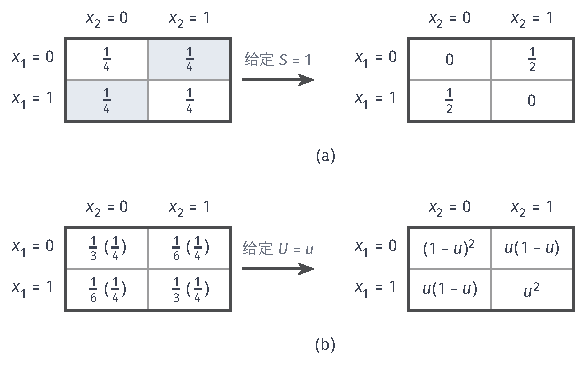
\includegraphics[width=98mm]{figures/07-probability/02-measure-theoretic-probability/tikz/cdis-ci-tables/figure.pdf}
  \caption{独立性随条件信息改变。(a)两枚独立公平硬币的联合概率表，浅蓝格子是事件$\{S=1\}$；给定$S=1$后只剩反对角线上的两格，$X_1$决定$X_2$。(b)随机硬币前两次抛掷的联合概率表，与各格边缘乘积（括号内）对照；给定$U=u$时表变为$u,1-u$的乘积表（右侧），条件独立而无条件不独立。}
  \label{fig:cdis-ci-tables}
\end{BookInlineFigure}

\paragraph{条件独立但不独立}
反方向用随机硬币。给定$U=u$时$X_1,X_2$独立，各以概率$u$为正面，所以$X_1\perp\!\!\!\perp X_2\mid U$。不给$U$时，由第~\ref{sec:cdis-chain}小节的公式，
\[
 \mathbb{P}(X_1=1,\ X_2=1)=\int_0^1u^{2}\,\mathrm{d}u=\frac13\neq\frac14=\mathbb{P}(X_1=1)\,\mathbb{P}(X_2=1).
\]
二者正相关，协方差为$\tfrac13-\tfrac14=\tfrac1{12}$，恰好是$\operatorname{Var}(U)$：两次抛掷共用同一个未知的正面概率，第一次的结果透露了$U$，于是影响对第二次的判断。

两个例子放在一起看。第一个例子中，$S$由$X_1,X_2$共同决定；把它加入条件，原本独立的两个量变得相关。第二个例子中，$U$同时影响$X_1,X_2$；把它从条件中去掉，原本条件独立的两个量变得相关。增加信息并不总是破坏独立：第二个例子中再给定$X_3$，即给定$(U,X_3)$，$X_1$与$X_2$仍然条件独立，因为给定$U$时三次抛掷相互独立。条件独立是$X$、$Z$与所给信息三者共同的性质，换了信息就要重新检查。

\paragraph{条件化与干预}
条件化回答的是“观测到$X_1=1$以后，对$X_2$的判断应当怎样修正”。随机硬币中，答案是把$\mathbb{P}(X_2=1)$从$\tfrac12$改成$\tfrac23$。另一个问题是：若有人不抛第一枚硬币，而是直接把它的记录写成正面，第二次抛掷的规律会怎样？这时硬币的正面概率$U$没有受到任何影响，第二次仍以$\tfrac12$的概率出现正面。

这两个问题的答案不同，而且第二个问题不能只靠联合分布回答。另一个模型是：第一次是公平硬币，第二次在第一次为正面时以$\tfrac23$、为反面时以$\tfrac13$出现正面。它与随机硬币的$(X_1,X_2)$有完全相同的联合分布，但在这个模型里改写第一次的记录，第二次正面的概率会变成$\tfrac23$。条件概率由联合规律决定；改变某个变量的产生方式以后会发生什么，还依赖产生数据的机制。研究这种操作的模型可参考\BookChapterRef{chap:causal-models-counterfactuals}{卷八第10章“因果模型与反事实”}。

\subsection{条件独立下的核复合}
\label{sec:cdis-composition}

设$X,Y,Z$都取值于标准Borel空间。已知给定$X$时$Y$的条件分布$K_{Y\mid X}$，以及给定$Y$时$Z$的条件分布$K_{Z\mid Y}$，能否得到给定$X$时$Z$的条件分布？一个自然的公式是先按$K_{Y\mid X}(x,\cdot)$抽出中间值$y$，再按$K_{Z\mid Y}(y,\cdot)$抽$z$，即对中间值积分。这个公式需要条件独立。

\begin{theorem}[核的复合]
\label{thm:cdis-composition}
设$X\perp\!\!\!\perp Z\mid Y$，$K_{Y\mid X}$与$K_{Z\mid Y}$分别是给定$X$时$Y$、给定$Y$时$Z$的正则条件分布。则
\begin{equation}
 L(x,C)=\int K_{Z\mid Y}(y,C)\,K_{Y\mid X}(x,\mathrm{d}y)
 \label{eq:cdis-composition}
\end{equation}
是给定$X$时$Z$的正则条件分布。
\end{theorem}

\begin{proof}
先说明$L$是概率核。固定$x$，$C\mapsto L(x,C)$非负、$L(x,\mathcal{Z})=1$；对两两不交的$C_n$，$K_{Z\mid Y}(y,\cup_nC_n)=\sum_nK_{Z\mid Y}(y,C_n)$，由单调收敛定理逐项积分，得到可数可加性。固定$C$，$y\mapsto K_{Z\mid Y}(y,C)$是有界可测函数，由定理~\ref{thm:cdis-kernel-product}第2条（被积函数只依赖$y$），$x\mapsto L(x,C)$可测。

再核对版本性质。固定$C$。依次用塔式法则（$\sigma(X)\subseteq\sigma(X,Y)$）、定理~\ref{thm:cdis-ci-markov}、正则条件分布$K_{Z\mid Y}$的定义，以及定理~\ref{thm:cdis-integral-representation}（对有界可测函数$y\mapsto K_{Z\mid Y}(y,C)$），得到
\[
 \begin{aligned}
 \mathbb{P}(Z\in C\mid X)
 &=\mathbb{E}\bigl[\mathbb{P}(Z\in C\mid X,Y)\bigm|X\bigr]
 =\mathbb{E}\bigl[\mathbb{P}(Z\in C\mid Y)\bigm|X\bigr]\\
 &=\mathbb{E}\bigl[K_{Z\mid Y}(Y,C)\bigm|X\bigr]\\
 &=\int K_{Z\mid Y}(y,C)\,K_{Y\mid X}(X,\mathrm{d}y)=L(X,C),
 \end{aligned}
\]
每个等号都几乎必然成立。
\end{proof}

式~\eqref{eq:cdis-composition}在有限状态时就是矩阵乘法。设$X$是房间的真实状态，$Y$是传感器读数，$Z$是传输到记录端的数值，都取$\{0,1\}$。读数只依据真实状态产生，记录只依据读数产生，转移矩阵为
\[
 \bm{W}_1=\begin{pmatrix}0.9&0.1\\0.2&0.8\end{pmatrix},\qquad
 \bm{W}_2=\begin{pmatrix}0.8&0.2\\0.3&0.7\end{pmatrix},
\]
第$i$行是给定上一级取值$i$时下一级的分布。

按第~\ref{sec:cdis-chain}小节的逐步构造，$Z$那一步的核只依赖$y$，所以$\mathbb{P}(Z\in C\mid X,Y)=\bm{W}_2$中第$Y$行在$C$上的和，它是$\sigma(Y)$可测的，于是也等于$\mathbb{P}(Z\in C\mid Y)$。由定理~\ref{thm:cdis-ci-markov}，$X\perp\!\!\!\perp Z\mid Y$。于是由式~\eqref{eq:cdis-composition}，给定$X$时$Z$的条件分布是
\[
 \bm{W}_1\bm{W}_2=\begin{pmatrix}0.9\cdot0.8+0.1\cdot0.3&0.9\cdot0.2+0.1\cdot0.7\\0.2\cdot0.8+0.8\cdot0.3&0.2\cdot0.2+0.8\cdot0.7\end{pmatrix}=\begin{pmatrix}0.75&0.25\\0.40&0.60\end{pmatrix}.
\]
真实状态为$0$时，记录正确的概率是$0.75$，由两条路径组成：读数正确且传输正确（$0.72$），读数错误且传输又出错（$0.03$）。图~\ref{fig:cdis-composition}(a)画出这些路径。

\begin{BookInlineFigure}
  \centering
  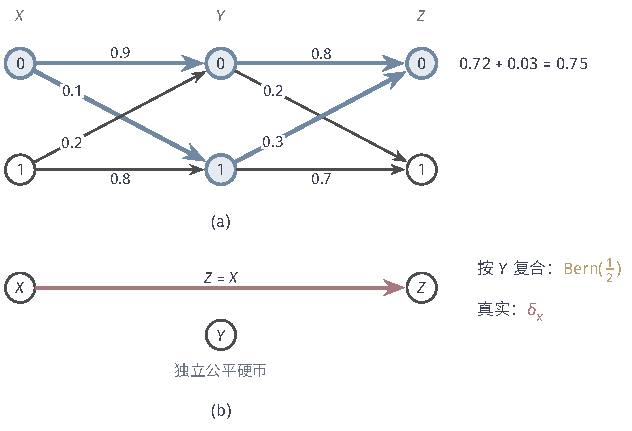
\includegraphics[width=107mm]{figures/07-probability/02-measure-theoretic-probability/tikz/cdis-composition/figure.pdf}
  \caption{核的复合。(a)$X\to Y\to Z$两级转移，边上是转移概率；从$X=0$到$Z=0$的两条路径（蓝）贡献$0.72$与$0.03$，合计$0.75$。(b)$Z=X$、$Y$为独立硬币时，按中间值$Y$复合得到$\operatorname{Bern}(\tfrac12)$（黄），而真实的条件分布是$\delta_x$（红）。}
  \label{fig:cdis-composition}
\end{BookInlineFigure}

\paragraph{条件独立不成立时}
复合公式不能直接用于任意三个随机变量。设$X,Y$是两枚独立的公平硬币，$Z=X$。给定$X$时$Y$仍是公平硬币；$Z=X$与$Y$独立，给定$Y$时$Z$也是公平硬币。按式~\eqref{eq:cdis-composition}复合，得到给定$X=x$时$Z\sim\operatorname{Bern}(\tfrac12)$；可是$Z=X$，真实的条件分布是$\delta_x$。错误在于$Z$与$X$的依赖并不经过$Y$：给定$Y$以后，$X$仍然完全决定$Z$，条件独立不成立。

复合公式对应的是一个两步构造：先有$X$，由$X$产生$Y$，再只由$Y$产生$Z$，依赖只通过中间变量传递。模型若按这种方式给出，条件独立由构造本身保证，复合可以放心使用；对已经给定的三个随机变量，必须先核对$X\perp\!\!\!\perp Z\mid Y$。
